\documentclass[bachelor, och, coursework]{SCWorks}
% параметр - тип обучения - одно из значений:
%    spec     - специальность
%    bachelor - бакалавриат (по умолчанию)
%    master   - магистратура
% параметр - форма обучения - одно из значений:
%    och   - очное (по умолчанию)
%    zaoch - заочное
% параметр - тип работы - одно из значений:
%    referat    - реферат
%    coursework - курсовая работа (по умолчанию)
%    diploma    - дипломная работа
%    pract      - отчет по практике
% параметр - включение шрифта
%    times    - включение шрифта Times New Roman (если установлен)
%               по умолчанию выключен
\usepackage{subfigure}
\usepackage{tikz,pgfplots}
\pgfplotsset{compat=1.5}
\usepackage{float}

%\usepackage{titlesec}
\setcounter{secnumdepth}{4}
%\titleformat{\paragraph}
%{\normalfont\normalsize}{\theparagraph}{1em}{}
%\titlespacing*{\paragraph}
%{35.5pt}{3.25ex plus 1ex minus .2ex}{1.5ex plus .2ex}

\titleformat{\paragraph}[block]
{\hspace{1.25cm}\normalfont}
{\theparagraph}{1ex}{}
\titlespacing{\paragraph}
{0cm}{2ex plus 1ex minus .2ex}{.4ex plus.2ex}

% --------------------------------------------------------------------------%


\usepackage[T2A]{fontenc}
\usepackage[utf8]{inputenc}
\usepackage{graphicx}
\graphicspath{ {./images/} }
\usepackage{tempora}

\usepackage[sort,compress]{cite}
\usepackage{amsmath}
\usepackage{amssymb}
\usepackage{amsthm}
\usepackage{fancyvrb}
\usepackage{listings}
\usepackage{listingsutf8}
\usepackage{longtable}
\usepackage{array}
\usepackage[english,russian]{babel}

%\usepackage[colorlinks=true]{hyperref}
\usepackage{url}

\usepackage{underscore}
\usepackage{setspace}
\usepackage{indentfirst} 
\usepackage{mathtools}
\usepackage{amsfonts}
\usepackage{enumitem}
\usepackage{tikz}
\usepackage{minted}
\setminted[py]{fontsize=\small, breaklines=true, style=bw, linenos}
\newcommand{\eqdef}{\stackrel {\rm def}{=}}
\newcommand{\specialcell}[2][c]{%
\begin{tabular}[#1]{@{}c@{}}#2\end{tabular}}

\renewcommand\theFancyVerbLine{\small\arabic{FancyVerbLine}}

\newtheorem{lem}{Лемма}

\begin{document}

% Кафедра (в родительном падеже)
\chair{теоретических основ компьютерной безопасности и криптографии}

% Тема работы
\title{Исследование моделей рекомендательных систем}

% Курс
\course{4}

% Группа
\group{431}

% Факультет (в родительном падеже) (по умолчанию "факультета КНиИТ")
\department{факультета КНиИТ}

% Специальность/направление код - наименование
%\napravlenie{09.03.04 "--- Программная инженерия}
%\napravlenie{010500 "--- Математическое обеспечение и администрирование информационных систем}
%\napravlenie{230100 "--- Информатика и вычислительная техника}
%\napravlenie{231000 "--- Программная инженерия}
\napravlenie{100501 "--- Компьютерная безопасность}

% Для студентки. Для работы студента следующая команда не нужна.
% \studenttitle{Студентки}

% Фамилия, имя, отчество в родительном падеже
\author{Окунькова Сергея Викторовича}

% Заведующий кафедрой
\chtitle{доцент, к.ф.-м.н.} % степень, звание
\chname{М.~Б.~Абросимов}

%Научный руководитель (для реферата преподаватель проверяющий работу)
\satitle{Доцент} %должность, степень, звание
\saname{И. И. Слеповичев}

% Руководитель практики от организации (только для практики,
% для остальных типов работ не используется)
%\patitle{к.ф.-м.н.}
%\paname{М.~Б.~Абросимов}

% Семестр (только для практики, для остальных
% типов работ не используется)
%\term{8}

% Наименование практики (только для практики, для остальных
% типов работ не используется)
%\practtype{преддипломная}

% Продолжительность практики (количество недель) (только для практики,
% для остальных типов работ не используется)
%\duration{4}

% Даты начала и окончания практики (только для практики, для остальных
% типов работ не используется)
%\practStart{30.04.2019}
%\practFinish{27.05.2019}

% Год выполнения отчета
\date{2023}

\maketitle

% Включение нумерации рисунков, формул и таблиц по разделам
% (по умолчанию - нумерация сквозная)
% (допускается оба вида нумерации)
% \secNumbering

%-------------------------------------------------------------------------------------------
\tableofcontents

\intro

    В последние несколько лет искусственный интеллект и нейронные сети стали все
    больше и больше влиять на нашу жизнь. Уже не существует человека, который
    не встречался с результатами работы нейронных сетей и машинного обучения.
    Таковой является выдача рекомендаций на разных сайтах в сети интернет.

    На сегодняшний день построение персонализированных рекомендаций является
    одним из самых перспективных и актуальных направлений машинного обучения.
    Его целью является повышения конверсии, среднего чека и улучшения опыта
    пользователя при использовании некоторого сервиса. В современном мире
    каждая компания, которая предоставляет доступ к контенту, как правило,
    имеет свою рекомендательную систему, поэтому с каждым годом количество
    решений в этой области растет все сильнее.

    Целью данной работы является разбор и сравнение подходов машинного
    обучения для данной задачи, а также изучение тенденций и перспектив развития 
    данной сферы в будущем.

\defabbr

\textit{Искусственный интеллект (АИ)} (англ. Artificial Intelligence) "--- это наука, описывающая создание машины или программы,
способной имитировать человеческое поведение для выполнения определенной задачи и обучаться
за счет полученной в результате работы информации.

\textit{Машинное обучение (МЛ)} (англ. Machine Learning) "--- это метод анализа данных, который автоматизирует построение аналитической 
модели.[1] Данная область ИИ воплощает в себе идею того, что машина способна обрабатывать полученные данные, анализировать их 
и на основе анализа обучаться с минимальным вмешательством человека.

\textit{Нейронная сеть (нейросеть, НС)}  (англ. Neural Network) "--- математическая модель и ее программная реализация, созданная
на основе модели биологических нейронных сетей (сетей нервных клеток организма).

\textit{Набор данных, выборка} (англ. dataset) "--- совокупность элементов, на которых проводят эксперимент.

\textit{Обучающая выборка} (англ. train dataset) "--- выборка, на которой обучают модели машинного обучения.

\textit{Валидационная выборка} (англ. validation dataset) "--- выборка, данные в которой не попали в обучающую выборку,
на которой измеряется качество прогнозирования модели на этапе обучения для контролирования этого процесса.

\textit{Тестовая выборка} (англ. test dataset) "--- выборка, на которой проверяется качество прогнозирования модели
после ее обучения.

\textit{Ансамбль}  (англ. ensemble) "--- набор из нескольких моделей, работающих параллельно или последовательно.

\textit{Бейзлайн} (англ. baseline) "--- простая модель, которая не требует большого количества ресурсов и с
результатами которой сравниваются более сложные модели.

\textit{Энкодер} (англ. encoder) "--- модель для представления определенной сущности в виде математического вектора.

\textit{Эмбеддинг} (англ. embedding) "--- сопоставление определенной сущности некоторому вектору, с помощью которого
можно представить эту сущность в математическом пространстве.

\textit{Холодный пользователь} "--- пользователь, у которого небольшая история взаимодействия
с сервисом.

\textit{Холодный объект} "--- объект, с которым взаимодействовало малое количество пользователей.

\textit{Матрица взаимодействий} "--- матрица, построенная на основе истории взаимодействия пользователя с
объектами, в которой строки - представляют из себя пользователя, столбцы объекты, а содержимое отражает
опыт взаимодействия пользователя с объектом (явный и неявный фидбэк).

\textit{Явный фидбэк} "--- обратная связь пользователя по взаимодействию с объектом, по которой можно точно
сказать получил ли пользователь положительный опыт или отрицательный (например оценка объекта).

\textit{Неявный фидбэк} "--- обратная связь пользователя по взаимодействию с объектом, по которой нельзя точно
сказать получил ли пользователь положительный опыт или отрицательный (например клик по объекту или время взаимодействия
с объектом).

\textit{Сингулярное разложение (SVD)} "--- определённого типа разложение прямоугольной матрицы,
позволяющее вычислять сингулярные числа матрицы, а также левые и правые сингулярные векторы матрицы.
Данное разложение имеет следующий вид:

\begin{equation}
    M_{n\times m} = U\Sigma V^*,
\end{equation}

где $\Sigma$  — матрица размера $m\times n$ с неотрицательными элементами, у которой элементы, лежащие на главной диагонали — это сингулярные числа (а все элементы, не лежащие на главной диагонали, являются нулевыми), а матрицы 
$U$ (порядка $m$) и $V$ (порядка $n$) — это две унитарные матрицы, состоящие из левых и правых сингулярных векторов соответственно (а
$V^*$ — это сопряжённо-транспонированная матрица к $V$).

\textit{Метод ближайших соседей} "--- простейший математический метод, основанный на расчете расстояния
в математическом пространстве от заданного объекта до других. В задачах рекомендации используется для поиска
схожих объектов к заданному путем выбора таких объектов, до которых расстояние от заданного наименьшее.
По стандарту расчет расстояние производится по формуле Евклида:

\begin{equation}
    d(x, y) = \sqrt{\sum_i^n (x_i - y_i)^2}.
\end{equation}

\textit{Градиентный бустинг} "--- архитектура, в основе которой лежит ансамбль, состоящий из недообученных деревьев,
работающих последовательно, где каждое новое дерево учится на ошибках предыдущих, за счет чего достигается высокая
скорость работы.

\textit{Случайные блуждания} (англ. random walk) "---  математический объект, известный как стохастический или случайный процесс, который описывает путь, состоящий из последовательности случайных шагов в каком-нибудь математическом пространстве.

\textit{A/B тестирование} "--- способ тестирования, при котором выборка пользователей делится на две статистически
схожие выборки, к которым применяются два разных алгоритма с целью сравнения результатов их работы в реальном времени.

\textit{Модель} "--- это алгоритм, который используется для предсказания значений целевой переменной на основе входных данных.
Она может быть представлена в виде математической формулы, графа или другой структуры, которая описывает зависимости между входными и
выходными данными.

\section{Теоретическая часть}
\subsection{Персонализированные рекомендательные системы}
Задача построения персонализированной рекомендательной системы заключается в том, чтобы построить такую рекомендательную
систему, которая на основе взаимодействий конкретного пользователя с определенным сервисом будет выдавать ему
уникальные и актуальные для него рекомендации. Такую задачу еще называют задачей ранжирования.

Важным аспектом персонализированных рекомендательных систем является баланс между персонализацией и разнообразием рекомендаций.
Слишком узкая персонализация может привести к тому, что пользователь не увидит новых товаров или услуг, а слишком широкая - к тому,
что он будет получать нерелевантные рекомендации.
\subsection{Модели}
Для решение задачи ранжирования существует множество подходов, которые обычно подразделяют на три типа:

\begin{enumerate}
    \item Основанные на схожести содержания объектов (content based фильтрация). При данном подходе пользователю рекомендуются
    объекты, которые похожи содержимым на те, с которыми он недавно взаимодействовал. При данном подходе сильно страдают
    метрики связанные с разнообразием рекомендуемых объектов, что является его большим минусом, так как в какой-то
    момент пользователю с большой вероятностью будет рекомендоваться то, что он уже видел.
    \begin{figure}[H]
        \centering
        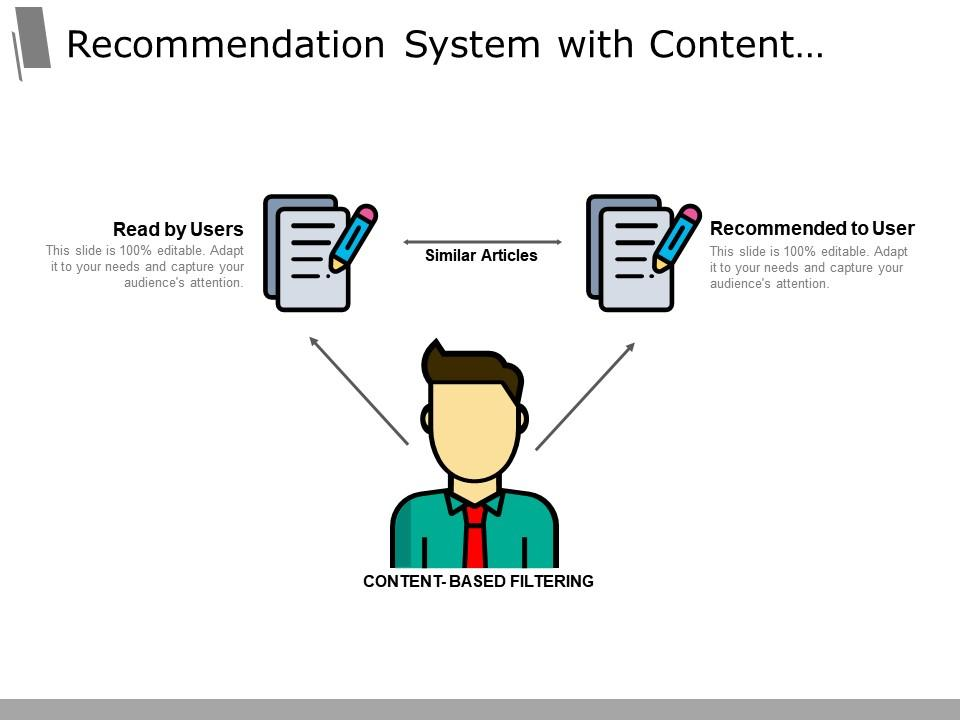
\includegraphics[width=0.65\textwidth]{pic/2}
        \caption{Принцип работы content based фильтрации[6]}
        \label{fig:img1}
    \end{figure}
    \item Коллаборативная фильтрация. Данные модели основаны на идеи поиска похожих пользователей (User based) или объектов (Item based)
    на основе истории взаимодействий. Главными минусами такого подхода является большее время на обучения модели и отсутствие учета содержимого объектов рекомендации.
    \begin{figure}[H]
        \centering
        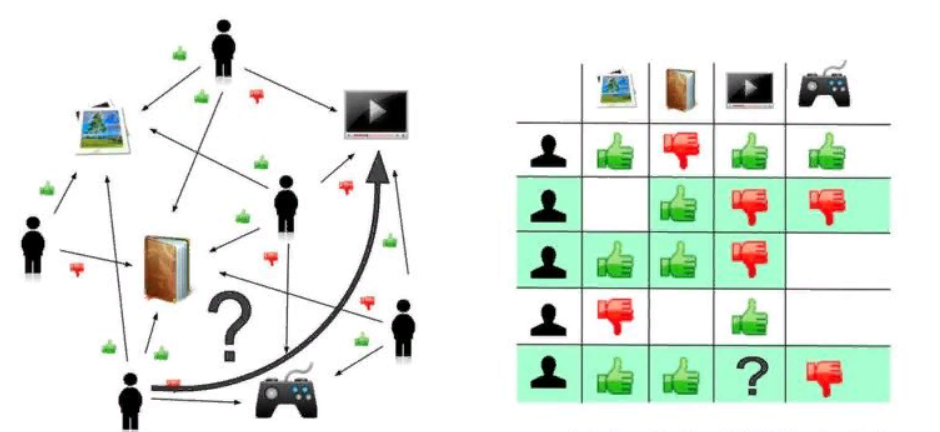
\includegraphics[width=0.7\textwidth]{pic/1}
        \caption{Принцип работы коллаборативной фильтрации[5]}
        \label{fig:img1}
    \end{figure}
    \item Гибридная фильтрация. Как понятно из названия, данные методы совмещают в себе предыдущие, сохраняя их сильные
    стороны, представляя из себя ансамбли из предыдущих моделей. Единственный минус таких моделей это необходимость 
    больше времени на обучения, что нивелируется более высокими метриками.
    \begin{figure}[H]
        \centering
        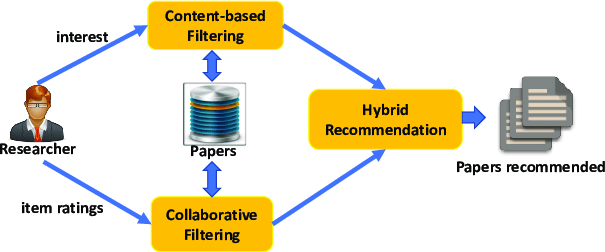
\includegraphics[width=0.7\textwidth]{pic/3}
        \caption{Принцип работы гибридной фильтрации[3]}
        \label{fig:img1}
    \end{figure}
\end{enumerate}

В данный промежуток времени первые два подхода являются хорошо изученными и модели, относящиеся к ним называются
моделями первого уровня. Эксперименты с гибридными архитектурами же продолжаются. Другими словами основное развитие
в сфера рекомендательных систем сегодня заключается в поисках такой архитектуры, которая сможет лучше всего использовать
результаты моделей первого уровня.

Стоит отметить, что выбор модели для ранжирования зависит не только от качества модели, но и от позиционирования
этой модели в сервисе. Т.е., например, если для сервиса необходима рекомендация объекта похожего на тот, с которым пользователь
взаимодействует в данный момент лучше всего подойдут модели, основанные на содержимом объекта.
\subsubsection{Рекомендация популярного}
Данная модель является хорошим бейзлайном для данного класса задач, а также хорошей моделью для построения
рекомендаций для холодных пользователей, так как не требует информации об истории взаимодействий пользователя.
Но это же и является главным минусом такого подхода: такие рекомендации будут являться неперсонализированными,
т.е. всем пользователям будут рекомендоваться одни и те же объекты, что чревато плохим качеством рекомендаций.

Данный подход можно улучшить за счет добавления простых правил. Например, рекомендации объектов популярных у
возрастной группы, к которой относится пользователь и т.д. Такой подход требует больше информации о пользователе,
но при этом качество рекомендаций будет гораздо выше. Однако, такая модель также является неперсонализированной,
при этом требует более тщательного анализа данных и проигрывает по качеству моделям, в основе которых лежит машинное
обучение.

Такой способ рекомендаций сложно отнести к какой либо из вышеописанных категории моделей, но результаты полученные
с помощью него часто также применяют для переранжирования рекомендаций.
\subsubsection{Модели, основанные на контенте}
Модели данного типа сильно зависят от самого контента, на рекомендацию которого нацелена система. В большинстве случаев
основная сложность построение таких систем ранжирования, заключается в поиске способов представления объектов в математическом
пространстве, чтобы вместе со степенью отличия росло и расстояние между объектами в этом пространстве. Иными словами
основная задача заключается в построение грамотных эмбеддингов объектов, а нахождение похожих объектов по ним уже не
составляет большой проблемы. Для этого подойдет простейший алгоритм поиска ближайших соседей.

\begin{figure}[H]
    \centering
    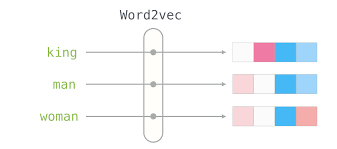
\includegraphics[width=0.7\textwidth]{pic/5}
    \caption{Пример получение эмбеддинга слов с помощью Word2Vec[7]}
    \label{fig:img1}
\end{figure}

Получения хороших эмбеддингов текстов является первым этапом задач NLP (Natural Language Processing), поэтому данный тип
контента представлять в виде вектора проще всего. Для этого используются такие энкодеры как BERT[18], Word2Vec[7], TFIDF, FastText[19] и другие.

Техника представления изображений является более сложной. Для получения их эмбеддинга обычно обучают некоторую модель сверточной нейронной сети для
классификации, чтобы взять результат с одного из ее последних слоев. Однако, совсем недавно миру были продемонстрированы такие модели
для работы с изображениями как VIT[20] и DeIT[21]. В основе их архитектуру лежит архитектура transformer, созданная изначально для NLP задач.
Сама архитектура моделей в данной работе не представляет такой интерес, как энкодинг изображения для подачи в нее. Изначально,
перед подачи изображения в сети ее представляют в виде вектора аналогично тексту. Для этого ее разбивают на несколько
частей, где преобразование каждой части эквивалентно преобразованию слова в NLP энкодере.

Метод работы с видеоданными в content based системах аналогичен работе с изображениями, так как видео представляет
из себя просто набор фрэймов (изображений). Поэтому видеоданные представляется либо вектором эмбеддингов всех его фреймов,
либо их суммой, либо их усреднением.

Хорошее представление же аудио данных является нерешенной задачей и по сей день. Существуют такие экспериментальные
методы как преобразование Фурье и спектрограммы. Однако большое количество работ в этой области показало не очень
хорошие результаты.
\subsubsection{Коллаборативная фильтрация}
В основе таких моделей лежит SVD разложение матрицы взаимодействий ($M$) пользователей с объектами на две матрицы ($U$ и $V$),
произведение которых вернет исходную матрицу взаимодействия. Однако вследствие того, что в матрице взаимодействий присутствует много
пропусков (т.к. не существует даже одного пользователя, которые полностью провзаимодействовал со всеми объектами
и наоборот), классические алгоритмы SVD разложения не используются, чтобы не потерять информацию о пока что отсутствующих
взаимодействиях. Для этой задачи используют поиск приближенного SVD разложения, который заключается в минимизации
функции 
\begin{equation}
    M_{n\times m} = UVmin(\sum_{i,j}(m_{i,j}-u_i \times v_j)),
\end{equation}
где $u_i$, $v_j$ строки и столбцы матриц $U$ и $V$ соответственно, $m_{i,j}$ - известные элементы матрицы $M$.
Минимизация может производиться различными математическими методами, например, с помощью градиентного спуска.

По факту полученные матрицы представляет из себя эмбеддинги пользователей и объектов, а вследствие того, что это приближение,
то на практике при их произведении получится приближенная матрица взаимодействия, т. е.

\begin{equation}
    U \times V \approx M.
\end{equation}

В следствие этого факта на местах пропусков появятся значения и при выдаче рекомендации нужно просто
выдать объекты, которые будут иметь максимальное значение в аппроксимированной матрице взаимодействия
и с которыми еще не взаимодействовал пользователь. Данный способ использования эмбеддингов является
гибридным, так как учитывает и схожесть пользователей и схожесть объектов, но является самым долгим,
так как операция умножения матриц имеет кубическую сложность.

По полученным эмбеддингам можно также производить поиск похожих пользователей или объектов (например с
помощью алгоритма ближайших соседей). Данные способы являются менее эффективными, но занимают меньше
времени для расчета рекомендаций нескольких пользователей ($O(km)$, где $k$ - это размер эмбеддинга,
а $m$ - количество объектов). Однако при расчете рекомендаций для всх пользователей будет получено
такое же время работы, как и при умножении матриц. Но даже в этом случае можно ускорить этот расчет
используя аппроксимацию ближайших соседей с помощью одной из следующих структур данных[17]:

\begin{enumerate}
    \item Граф.
    \item Дерево.
    \item Хэш корзины.
\end{enumerate}

Главным минусом коллаборативной фильтрации является невозможность ее применения для получения эмбеддингов холодных
пользователей и объектов. Но существуют некоторые алгоритмы, которые по признакам пользователя или объекта,
могут выдавать хороший эмбеддинг. Так, например, сервис spotify по спектрограмме музыки с помощью нейронных сетей
генерирует ее эмбеддинг, за счет чего происходит продвижение композиций малоизвестных исполнителей[16].

\subsubsection{Гибридные модели}
Обычно такие модели представляют из себя ансамбль, где на первом уровне находятся вышеописанные модели,
генерирующие параллельно списки рекомендованных объектов для пользователей и признаки в виде эмбеддингов
пользователь, объектов и содержимого объектов, а на втором некоторая модель занимается переранжированием объектов в этом списке.
Такая модель чаще всего представляет из себя классификатор, который выдает вероятность того, что пользователь провзаимодействует
с объектом. Такая архитектура позволяет не только получить дополнительные признаки, но и сократить время
на обучения и выдачу прогноза классификатора. При этом подход с классификатором является неединственным.
На смену ему приходят более сложные механизмы, которые показывают результаты лучше. Например, социальные
сети на основе результатов моделей первого уровня строят граф и используют проход по нему с помощью
алгоритмов случайных блужданий.

\begin{figure}[H]
    \centering
    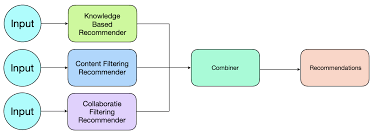
\includegraphics[width=0.6\textwidth]{pic/4}
    \caption{Двухуровневая архитектура[4]}
    \label{fig:img1}
\end{figure}


В данной работе будут рассмотрена только классическая архитектура с классификатором в виде механизма
переранжирования. Такая архитектура учится следующим образом: сначала происходит обучение моделей первого уровня,
затем находится пример положительного взаимодействия пользователя
с объектом и для этого примера этими моделями генерируется еще несколько примеров отрицательного
взаимодействия. Таким образом генерируется большая конечная выборка, после чего на ней происходит обучение
модели второго уровня.

В качестве переранжирующей модели можно использовать любой классификатор, но лучше себя показывают архитектуры
градиентного бустинга и нейронные сети, так как первые хорошо и быстро работают с большим количеством признаков,
а вторые можно очень гибко настроить с помощью кропотливого подбора слоев.

\subsection{Оценка качества рекомендательной системы}

Как и в других сферах машинного обучения, оценка качества рекомендаций проходит в два этапа:

\begin{enumerate}
    \item Оценка в офлайне на данных, которые уже существуют. На данном этапе принимается решение о
    целесообразности применения нового подхода в реальных условиях. За счет этого сразу отсекаются
    модели, которые выдают плохие метрики.
    \item Оценка в онлайне с помощью A/B тестирования. На данном этапе уже идет сравнение с используемой
    в данной момент моделью, чтобы понять на сколько лучше/хуже работает новая модель.
\end{enumerate}

Стоит отметить, что не всегда высокие метрики в онлайне хорошо коррелируют с высокими метриками в офлайне.
При этом модели рекомендательных систем больше всего подвержены ухудшению качества со временем, чем их собратья
из других сфер, из-за чего их нужно переобучать раз в какой-то период, что тоже влияет на принятие решения
об их имплементации в качестве новых основных моделей.

Существует множество метрик, по которым сравнивается качество работы моделей. Основными из них являются 
MAP$@k$ (Mean Average Precision at $k$) и nDCG$@k$ (normalized Discounted Cumulative Gain at $k$). Они обе принимают значения в диапозоне [0,1],
где чем больше значение, тем лучше работа модели, и показывают
насколько хорошо ранжирование результатов соответствует предпочтениям пользователя, а разница между ними заключается
в том, что первую метрику используют в случае бинарных значений эталонной релевантности, а вторую в случае
небинарных.

Существуют также более продвинутые метрики, которые учитывают уникальность и полноту охвата рекомендаций.

\subsubsection{Mean Average Precision at k}
Пусть архитектура выдает k элементов в качестве рекомендации. В этом случае самой простой метрикой, которую
можно рассчитать для одного примера будет precision at k (p$@k$):

\begin{equation}
    \text{p}@k = \frac{\text{количество релевантных элементов}}{k}.
\end{equation}

Проблема данной метрики заключается в том, что она не учитывает позиции элементов в топе. Так две модели, которые
выдают одну релевантную рекомендацию будут иметь одинаковые метрики, даже, если первая модель выдает релевантную
рекомендацию на первом месте топа, а вторая на последнем. Очевидно, что в данном случае вторая модель проигрывает
первой по качеству.

Для того, чтобы подобной проблемы не возникало была создана метрика average precision at $k$ (ap$@k$):

\begin{equation}
    \text{ap}@k = \frac{1}{k}\sum_{i=1}^{k}r_i\text{p}@i,
\end{equation}

где $r_i$ принимает значение 1, в случае если $i$ элемент топа является релевантным, и 0 в обратном случае.

Выше описанные метрики применяются для оценки качества рекомендаций для одного пользователя. Для того, чтобы
вычислить качество ранжирования для $n$ пользователей берут среднее от суммы оценок ap$@k$ для них. Данная метрика
и называется mean average precision at $k$ и имеет формулу:

\begin{equation}
    \text{map}@k = \frac{1}{n}\sum_{i=1}^{n}\text{ap}@k_j.
\end{equation}

\subsubsection{Normalized Discounted Cumulative Gain}
В случае, если эталонные значения являются небинарными (например, оценки объектов), то лучше использовать
данную метрику. Она вычисляется по следующей формуле

\begin{equation}
    \text{nDCG}@k = \frac{\text{DCG}@k}{\text{IDCG}@k},
\end{equation}
где DSG@k вычисляется путем суммирования релевантностей всех результатов, учитывая их порядок в списке путем домножения релевантности элемента на вес равный обратному логарифму номера позиции, т.е.

\begin{equation}
    \text{DCG}@k = \sum_{i=1}^p\frac{2^{r_i} - 1}{log_2(i+1)},
\end{equation}
а IDCG$@k$ вычисляется аналогично DCG$@k$, но с учетом идеального порядка результатов.
\section{Практическая часть}
\subsection{Описание инструментов для программной реализации}
В качестве языка программирования для данной работы был выбран Python 3.10.10, потому что на сегодняшний день данный язык программирования он является самым привлекательным
решением для работы с глубоким обучением, имея только две хорошие альтернативы в лице разрабатываемого в данный момент языка Mojo и давно существующего языка R, рассчитанным больше на статистический анализ. Это связано не только с простотой работы с языком, но и с большим списком
библиотек, созданных специально для машинного обучения.

Чтобы проводить эксперименты с моделями и анализ данных была использована платформа Jupyter Notebook. С помощью этой платформы создается локальный сервер, на котором можно работать
с файлами с расширением .ipynb. Плюсом таких файлов является возможность запускать не весь код, написанный на языке Python, а лишь его части, хранящиеся в отдельных ячейках.
Это очень удобно, потому что весь код можно хранить в одном файле и запускать только необходимые в данный момент его части, за счет чего становится проще отлаживать конечную программу,
а также проводить эксперименты с данными.

Для визуализации, анализа и предобработки данных были использованы библиотеки matplotlib[22], seaborn[23] и pandas[24]. Первые две являются лучшим простым инструментом для визуализации данных
на данный момент не только в пределах проектов на языка python. Pandas же является практически безальтернативным решением для работы с табличными данными разных форматов, позволяя
не только интерпретировать их в понятный человеку вид, но и удобно анализировать их статистические свойства.

Для работы с моделями были использованы библиотеки implicit[25] и LightFM[26], которые содержат модели для построения рекомендательных систем, разных типов.

\subsection{Описание набора данных}
В качестве основной выборки были использованы данные, предоставленные компанией H\&M для kaggle соревнования по построению рекомендательной системы.[27] Данная выборка
представляет из себя три таблицы, записанные в формате CSV: таблицу пользователей (customres.csv), содержащую в себе признаки 1371980 пользователей, таблицу объектов (articles.csv),
содержащую в себе признаки 105542 товаров магазина, и таблицу взаимодействий (transactions.csv), содержащую в себе факты покупки товаров пользователями.

\subsection{Анализ данных}
Для построения хорошей рекомендательной системы необходимо хорошо понимать специфику данных, которые для этого используются. Поэтому первым этапом данной задачи является глубокий анализ данных.
\subsubsection{Таблица пользователей}
Таблица пользователей содержит в себе следующие атрибуты: customer_id, FN, Active, club_member_status, fashion_news_frequency, age, postal_code.

В результате анализа было замечено, что признаки FN и Active имеют много null значений. При выводе на экран уникальных значений в этих колонках видно, что эти колонки содержат только значения 1 и null, следовательно null значения можно заполнить нулем.

При дальнейшем анализе становится очевидно, что эти колонки очень хорошо коррелируют друг с другом, а это значит, что одну из них можно удалить. Выбор пал на колонку FN, так как не очень понятна, ее смысловая нагрузка.

В колонке age не так много пропусков. При этом распределение далеко от нормального. Минимальный возраст пользователя - 16. Скорее всего это возраст, с которого можно зарегистрироваться. Максимальный возраст пользователя - 99 лет, а так же много пользователей старше 50 даже больше, чем младше 20. Похоже на то, что многие люди при регистрации ставят не свой настоящий возраст. Матожидание возраста равно 36, при этом мода равна 21, поэтому для заполнения пропущенных значений было принято решение использовать моду.
\begin{figure}[H]
    \centering
    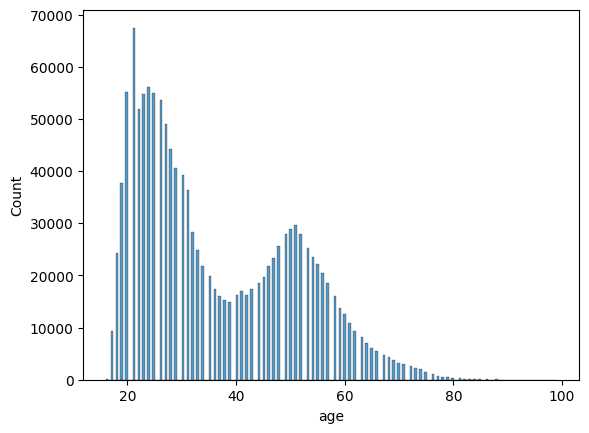
\includegraphics[width=0.8\textwidth]{pic/6}
    \caption{Распределение пользователей по возрасту в исходных данных}
    \label{fig:img1}
\end{figure}

Для создания более качественного бейзлайна было принято решение в дальнейшем использовать не возраст пользователя, а возрастную группу: 16-19, 20-40, 41-60, 60+. Таким образом распределение нового признака
выглядит более похоже на нормальное.

\begin{figure}[H]
    \centering
    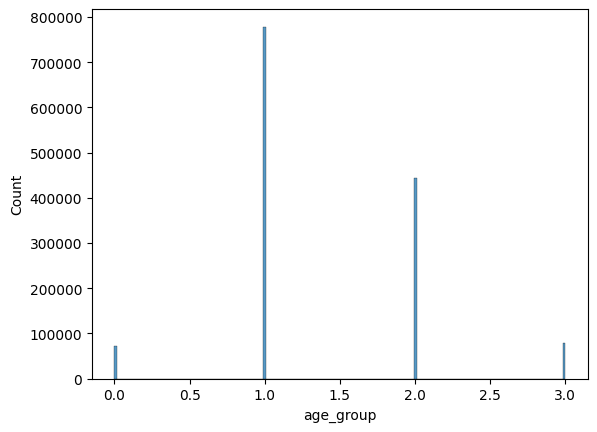
\includegraphics[width=0.76\textwidth]{pic/7}
    \caption{Распределение пользователей по возрастным группам (0 "--- 16-19, 1 "--- 20-40, 2 "---41-60, 3 "---60+)}
    \label{fig:img1}
\end{figure}

Пропуски в колонках fashion_news_frequency и club_member_status были заполнены по смыслу самих колонок: очевидно, что на месте пропусков должна содержаться информация об отсутствии подписки на новости магазина и отсутствии членского статуса. Помимо этого можно заметить, что в колонке fashion_news_frequency есть значения NONE и None. Вероятнее всего это одна и та жа категория значений, поэтому значение None было преобразовано в значение NONE.

Холодных пользователей очень много. Так 10\% пользователей имеет всего 1 покупку, 32\% имеют менее 5 купленных товаров, а меньше 10 товаров имеют 50\% пользователей. Будем считать, что пользователь является холодным, если он купил менее 5 товаров.

\subsubsection{Таблица объектов}
Таблица объектов содержат в себе следующие атрибуты: article_id, product_code, prod_name, product_type_no, product_type_name,
product_group_name, graphical_appearance_no, graphical_appearance_name, colour_group_code, colour_group_name, perceived_colour_value_id
perceived_colour_value_name, perceived_colour_master_id, perceived_colour_master_name, department_no, department_name,
index_code, index_name, index_group_no, index_group_name, section_no, section_name, garment_group_no, garment_group_name,
detail_desc.

Менее половины процента значений являются пропущенными в колонке detail_desc. Их можно просто заполнить пустой строкой.

В таблице много признаков, которые хорошо коррелируют друг с другом, однако они в основном представляют из себя пару имени какой-то категории и номера этой категории.

\begin{figure}[H]
    \centering
    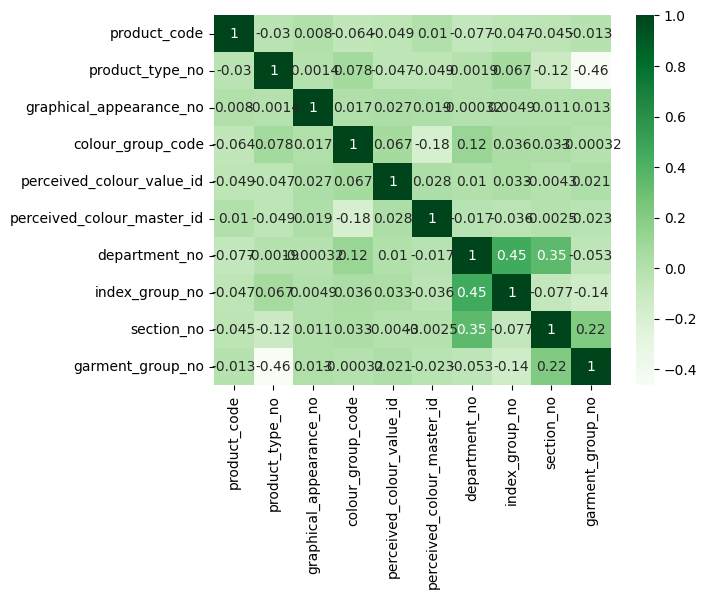
\includegraphics[width=0.9\textwidth]{pic/8}
    \caption{График корреляции признаков}
    \label{fig:img1}
\end{figure}

В каталоге магазина 131 уникальная категория товара. Больше всего таких товаров как трусы, платья, свитеры, футболки и топы, причем разрыв между первым и пятым местом почти в 3 раза. Можно заметить, что все, кроме свитеров, это вещи на любой сезон и легкие вещи, рассчитаны на весенний-летний сезон.Самыми редкими товарами являются специфические товары несвойственные магазину одежды: поясная сумка, ходунки, удлинитель бюстгальтера, деревянные шары, полотенце, швейный набор, мешок для стирки, брелок, повязка на голову, подушка, одеяло, спрей для одежды. Интересно насколько сильно количество товара определенной категории в каталоге будет коррелировать с продажами товаров из этих категорий. 

Помимо этого товары сгруппированы по 19 группам. Распределение этих групп стандартное для магазинов такого типа: больше всего обычной одежды, меньше всего специфических товаров, например средств для заботы об одежде.

Также при анализе товаров интерес вызвала колонка index_group_name.
В ней содержится информация о том, к какой коллекции принадлежит товар: мужская, женская, детская или унисекс(спортивная и разделяемая). Сама по себе она не несет большой интерес, однако с помощью нее позже при анализе транзакций можно будет сделать предположение о поле человека и о наличие у него детей в семье. Однако, даже в чистом виде с помощью данных в ней можно сделать предположение, что целевая аудитория данного магазина женщины и люди с детьми, так как товаров чисто для этих групп намного больше, чем чисто мужских товаров.

В аналогичном ключе интерес представляют колонки, связанные с цветом одежды. С помощью них также в связке с таблицей транзакций можно сделать предположение о любимом цвете пользователя. Однако, стоит отметить, что данное предположение будет являться менее точным, чем предыдущие.

В каталоге очень много холодных товаров. Конечно, сложно определить оптимальное значение покупок, начиная с которых товар будет называться холодным, поэтому было принято решение в целях анализа попробовать несколько разных значений. В результате получается, что для 10 20\% товаров будут являться холодными, для 50 - 45\%, для 100 - 57\%. Это может очень сильно сказаться на качестве работы моделей (особенно это актуально для матричных разложений), в результате чего более редкие товары будут рекомендоваться очень редко, если вообще будут.

\subsubsection{Таблица взаимодействий}
Таблица взаимодействий содержат в себе следующие атрибуты: t_dat, customer_id, article_id, price, sales_channel_id.

Сама по себе данная таблица не очень интересна в плане анализа данных, однако с помощью нее можно создать много признаков для объектов и пользователей, что уже отмечалось выше.

Однако при скудности таблицы на полезные для анализа признаки, с помощью нее удалось проанализировать распределение продаж по датам. На рисунке видно, что видно, что оно даже
близко неравномерное. Однако простой анализ дат не дает много информации. Более целесообразно провести анализ по месяцам и сезонам.

\begin{figure}[H]
    \centering
    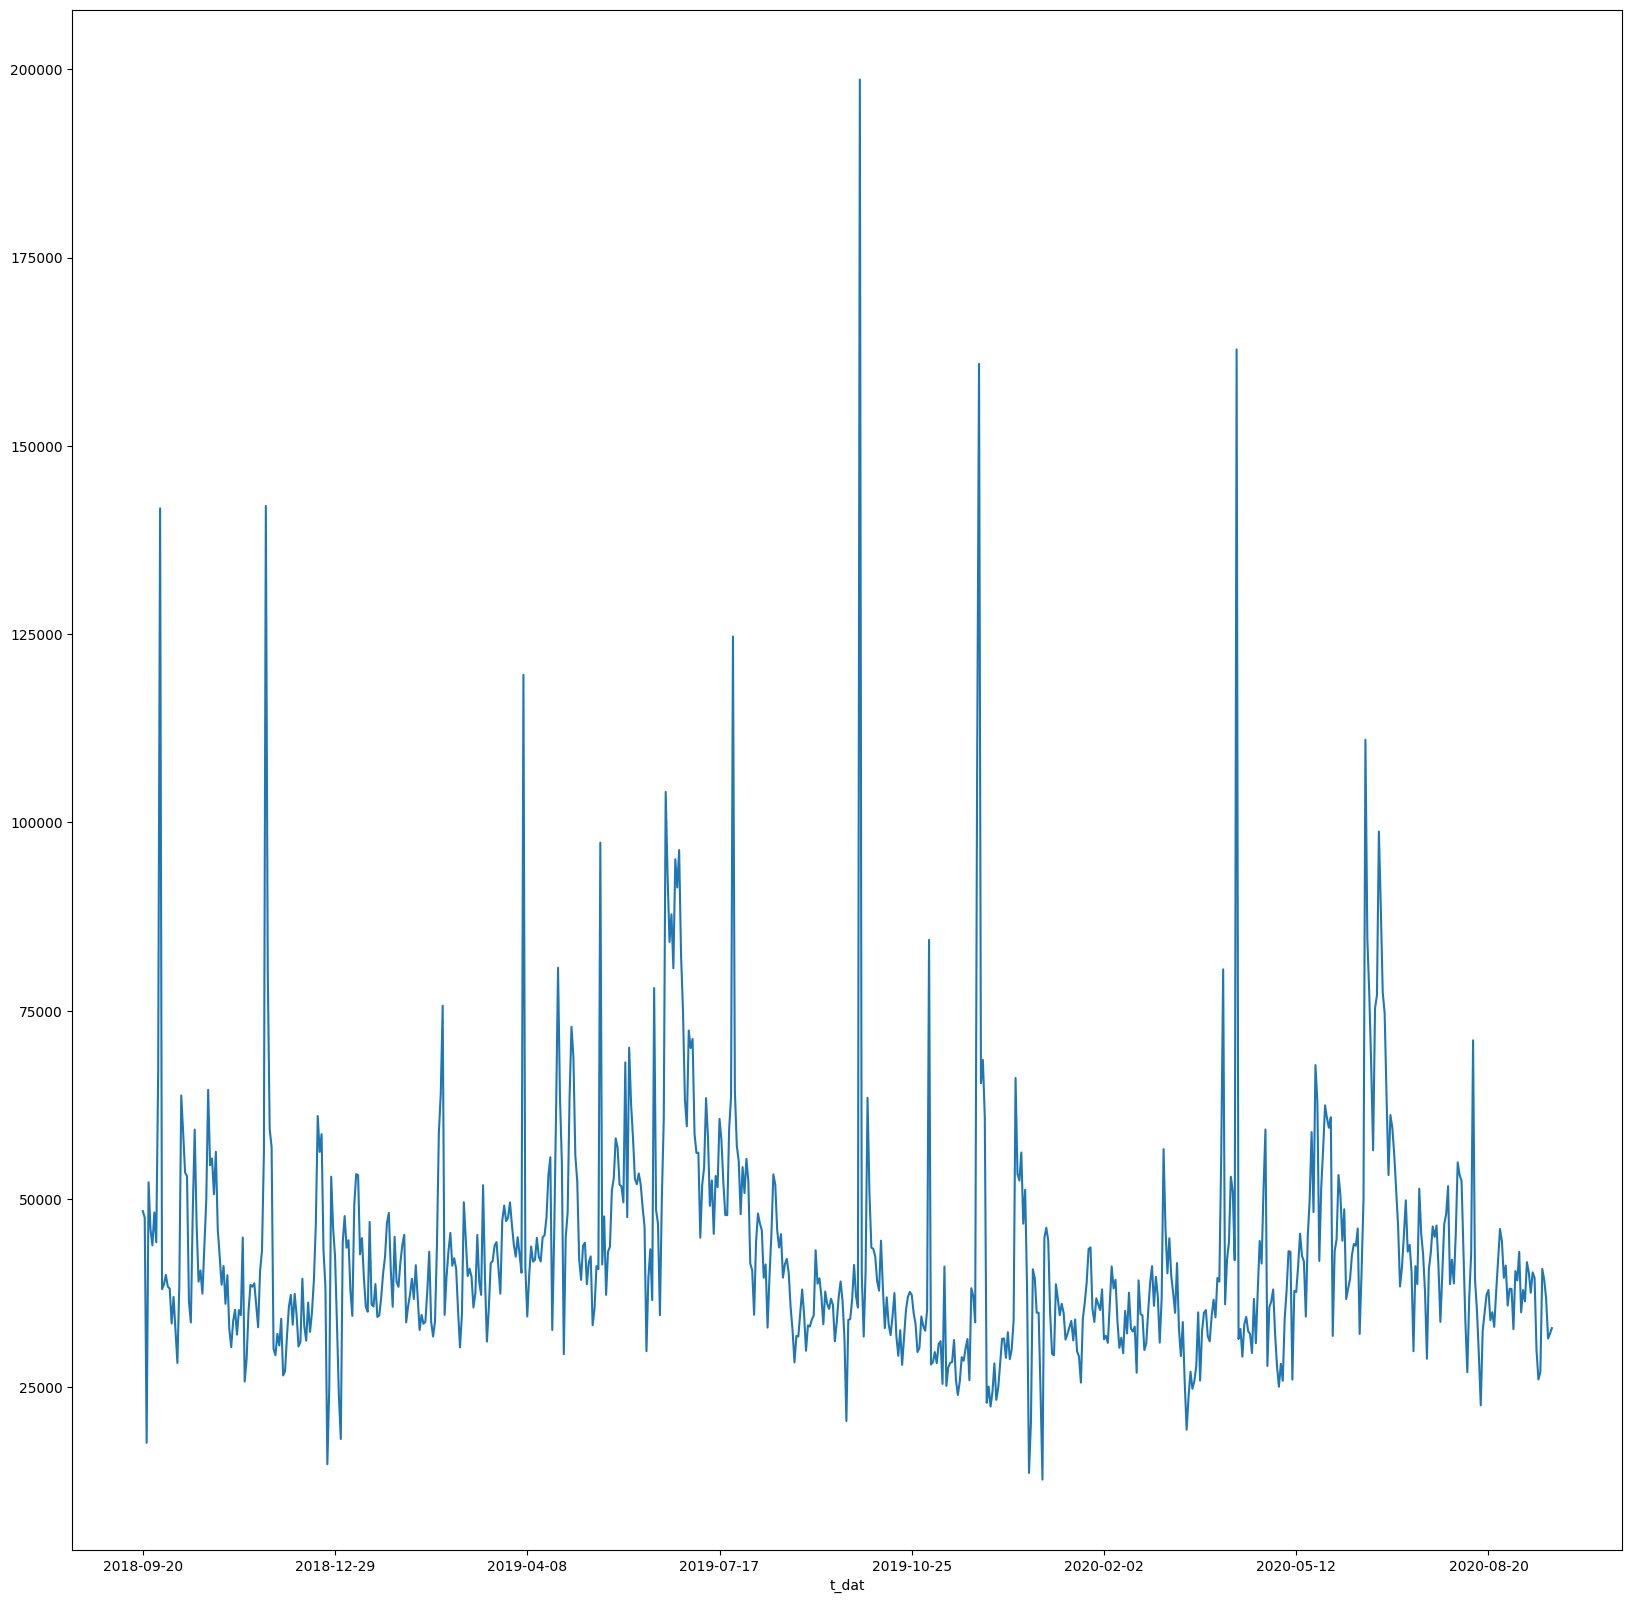
\includegraphics[width=0.8\textwidth]{pic/9}
    \caption{Распределение взаимодействий пользователей с товарами по датам}
    \label{fig:img1}
\end{figure}


\subsubsection{Генерация новых признаков и их анализ}

Теперь с помощью таблицы транзакций и других двух таблиц можно создать новые признаки и проанализировать их. 

В первую очередь можно получить информацию о сезоне, в котором объект имеет большую актуальность для покупки. В результате получается, что большинство товаров каталога имеет высокий спрос осенью, а меньше всего весной, хотя в целом больше всего покупок совершается летом.

\begin{figure}[H]
    \centering
    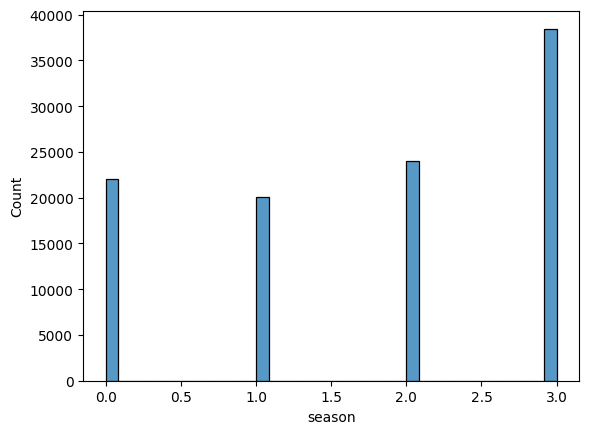
\includegraphics[width=0.8\textwidth]{pic/10}
    \caption{Распределение продаж товаров по сезонам}
    \label{fig:img1}
\end{figure}

Можно попробовать угадать пол человека по его покупкам(если человек покупает больше вещей из женской коллекции, то скорее всего это женщина и наоборот). Таким образом, построив распределение по полученному признаку, можно заметить, что женщин намного больше, чем мужчин.

\begin{figure}[H]
    \centering
    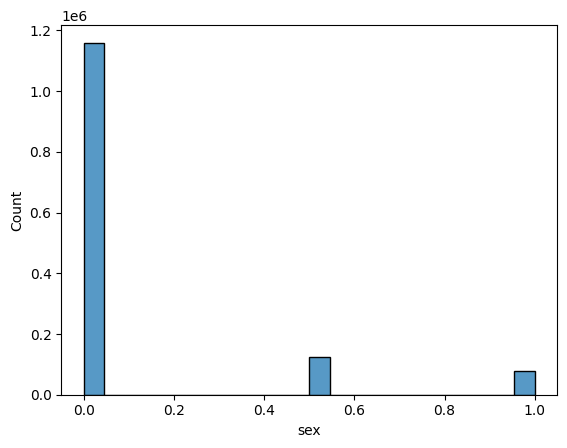
\includegraphics[width=0.7\textwidth]{pic/11}
    \caption{Распределение пользователей по полу (0 - женский, 1 - мужской, 0.5 - не удалось определить)}
    \label{fig:img1}
\end{figure}

Можно попробовать также угадать наличие у человека ребенка по его покупкам. Если у человека есть покупки из детской коллекции, то вероятнее всего у него есть ребенок. Проведя анализ данного распределения, становится понятно, что большинство пользователей не покупают детскую одежду вовсе. Таких пользователей примерно в 6 раз меньше, чем пользователей с детьми.

\begin{figure}[H]
    \centering
    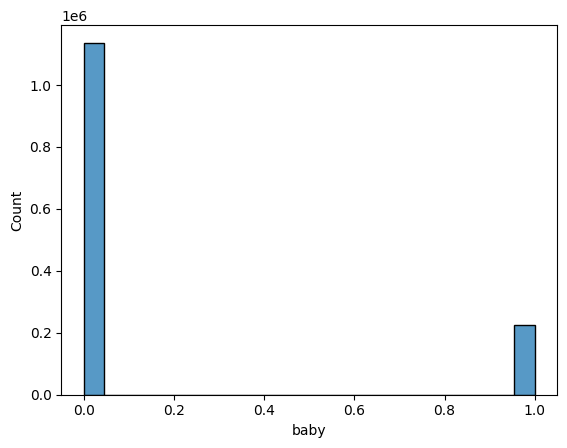
\includegraphics[width=0.6\textwidth]{pic/12}
    \caption{Распределение пользователей по наличию ребенка}
    \label{fig:img1}
\end{figure}

Помимо этого можно определить целевую возрастную аудиторию товара по его покупкам. Проанализировав данное распределение можно сделать вывод, что целевая аудитория магазина люди 20-40 лет, так как в каталоге много товаров для данной целевой группы. А вот для остальных групп товаров во много раз меньше. Так на втором месте находятся товары, целевая группа которых 40-60 лет, но при этом их в 4 раза меньше, чем для предыдущей целевой группы.

\begin{figure}[H]
    \centering
    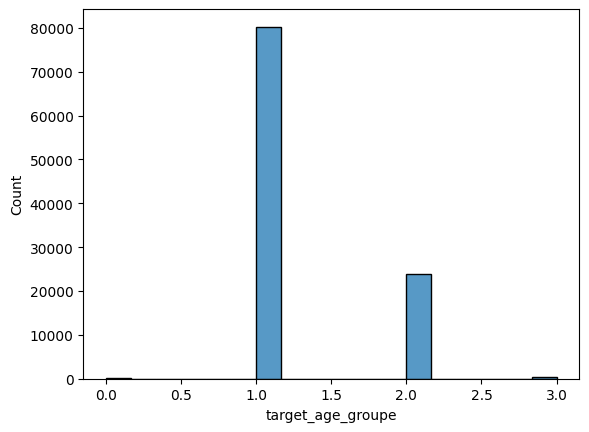
\includegraphics[width=0.8\textwidth]{pic/13}
    \caption{Распределение товаров по возрастной группе (0 "--- 16-19, 1 "--- 20-40, 2 "---41-60, 3 "---60+)}
    \label{fig:img1}
\end{figure}

\subsection{Используемые модели}
В рамках практической части данной работы были проведены эксперименты со всеми типами моделей, описанных в теоретической части,
которые выступают в виде моделей первого уровня: от рекомендации популярного, до гибридных моделей первого уровня.

В качестве бейзлайн модели была взята рекомендация популярного, который дальше был модифицирован с помощью нескольких простых правил:
рекомендации популярного относительно целевой группы пользователя и его пола. Так же была попытка делить пользователей по наличию ребенка,
но ни один товар для детей не попал в топ популярного, поэтому данная идея была отброшена.  

В качестве модели, основанной на контенте была взята модель tf-idf из библиотеки implicit. Несмотря на то, что она основана на
истории взаимодействий пользователей с объектами, она имеет иной подход, чем матричное разложение и считается content based моделью,
где контентом и являются эти взаимодействия.

Для матричного разложения были использованы модели ALS из библиотеки implicit и LightFM из одноименной библиотеки.
Причем LightFM может также являться гибридной, так как это разложение может учитывать признаки пользователей и объектов. 

\subsection{Процесс обучения}
Обучение всех моделей выполнялось в IDE Visual Studio Code на макбуке с системой MACOS на процессоре M1. 

В файле utils.py находится код для класса model, чтобы все модели имели общий интерфейс обращения, а также вспомогательные функции для оценки
качества моделей и разбиения данных на тренировочную и валидационную выборку.

В файле baseline.py содержится код для выдачи предсказаний с помощью бейзлайна. В файле rule_recommendation.py находится
код улучшенного бейзлайна. В файле tf_idf_recommender.py находится код для обучения TF IDF модели и выдачи ей предсказания.
В файле ALS_recommender.py находится код для аналогичных целей ALS модели. Аналогичный смысл имеет файл lightfm_recommender.py
для модели LightFM.

\subsection{Результаты обучения}
В качестве целевой метрики была выбрана метрика MAP$@k$, так как данная метрика является целевой в данном соревнование.
Валидация моделей проводилась на последней неделе тренировочной выборки. А в качестве тестовой использовались закрытые данные,
на которых тестовая система соревнования оценивает качество прогноза моделей. Которая в свою очередь поделена на две части в
соотношении 1 к 99. Ее наименьшая часть называется public, а наибольшая "--- private, за счет чего можно сравнить скорость
деградации моделей.

Результаты обучения моделей приведены в таблице 1.

\begin{table}[H]
    \begin{tabular}{|l|l|l|l|l|l|l|}
    \hline
                     & baseline & rules   & TF IDF  & ALS     & LightFM & LightFM (гибр)    \\ \hline
    valid score      & 0.002161 & 0.00263 & 0.00295 & 0.00675 & 0.00452 & 0.00303           \\ \hline
    public score     & 0.0015   & 0.00231 & 0.00174 & 0.014   & 0.00596 & 0.00074           \\ \hline
    private score    & 0.00161  & 0.00267 & 0.00207 & 0.01417 & 0.00586 & 0.00077           \\ \hline
    \end{tabular}
    \end{table}

\subsection{Вывод}
По результатам, которые выдали модели можно сделать следующие выводы:
\begin{enumerate}
    \item Модели, основанные на рекомендации популярного очень быстро деградируют, однако этот минус нивелируется
    тем, что их не нужно обучать. Достаточно просто рассчитывать, какие товары находятся в тренде в данный момент времени
    с помощью одного запроса в базу данных.
    \item Усложнив запрос в базу данных несколькими простыми правилами, можно сильно поднять качество бейзлайна.
    \item Модели матричной факторизации дают лучшие метрики относительно любых моделей первого уровня, однако работают плохо
    с холодными пользователями и объектами.
    \item Гибридные модели первого уровня показывают себя намного хуже, чем любые другие модели первого уровня, при этом усложняя
    программную реализацию и расходуют больше времени на обучение.
\end{enumerate}

\conclusion 
В теоретической части данной работы были рассмотрены основные понятия, алгоритмы и принципы построения рекомендательных систем, а также способы оценки их качества.
Были описаны понятия моделей первого и второго уровня разных типов, в связи с чем были рассмотрены таки понятия как эффективное представление разных типов данных в
машинном обучение, матричное разложение и эффективная аппроксимация хорошо известных алгоритмов ML.

В практической части на примере kaggle соревнования было проведено обучение моделей первого уровня и сравнение результатов с целью нахождения их плюсов и минусов
в реальных условиях. Помимо этого были проанализированы исходные данные, на основе чего были созданы более эффективные признаки объектов и пользователей с целью
улучшения качества прогноза алгоритмов.

\begin{thebibliography}{99}
    \bibitem{1}
    Пять технологий искусственного интеллекта, о которых вам нужно знать [Электронный ресурс] – URL: https://www.sas.com/ru_ru/insights/articles/analytics/five-ai-technologies.html (дата обращения 27.04.2021) - Загл. с экрана. Яз. рус.
    \bibitem{2}
    Нейронные сети для начинающих. Часть 1 [Электронный ресурс] – URL: https://habr.com/ru/post/312450/ (дата обращения 13.05.2022) - Загл. с экрана. Яз. рус.
    \bibitem{3}
    Verma Y. <<A Guide to Building Hybrid Recommendation Systems for Beginners>> [Электронный ресурс] – URL: https://analyticsindiamag.com/a-guide-to-building-hybrid-recommendation-systems-for-beginners/ (дата обращения 01.05.2023) - Загл. с экрана. Яз. англ.
    \bibitem{4}
    Building a hybrid recommendation system for Jokes recommendations [Электронный ресурс] – URL: https://www.oreilly.com/library/view/advanced-machine-learning/9781838641771/0aa25981-d582-4347-9928-2d967133822e.xhtml (дата обращения 01.05.2023) - Загл. с экрана. Яз. англ.
    \bibitem{5}
    Коллаборативная фильтрация простыми словами [Электронный ресурс] – URL: https://lala.lanbook.com/kollaborativnaya-filtraciya-prostymi-slovami (дата обращения 01.05.2023) - Загл. с экрана. Яз. рус.
    \bibitem{6}
    Recommendation system with content based filtering [Электронный ресурс] – URL: https://www.slideteam.net/recommendation-system-with-content-based-filtering.html (дата обращения 01.05.2023) - Загл. с экрана. Яз. англ.
    \bibitem{7}
    Word2vec в картинках [Электронный ресурс] – URL: https://habr.com/ru/articles/446530/ (дата обращения 01.05.2023) - Загл. с экрана. Яз. рус.
    \bibitem{8}
    Ермилов Д. <<Рекомендательные системы: продвинутые алгоритмы>> [Электронный ресурс] – URL: https://www.bigdataschool.ru/blog/recommender-systems-advanced-algorithms.html (дата обращения 01.05.2023) - Загл. с экрана. Яз. рус.
    \bibitem{9}
    Рекомендательные системы: что это и как работает алгоритм рекомендаций [Электронный ресурс] – URL: https://mindbox.ru/academy/education/rekomendatelnye-sistemy/ (дата обращения 01.05.2023) - Загл. с экрана. Яз. рус.
    \bibitem{10}
    Метод ближайших соседей [Электронный ресурс] – URL: http://www.machinelearning.ru/wiki/index.php?title=Метод_ближайшего_соседа (дата обращения 01.05.2023) - Загл. с экрана. Яз. рус.
    \bibitem{11}
    A/B тест — это просто [Электронный ресурс] – URL: https://habr.com/ru/articles/233911/ (дата обращения 01.05.2023) - Загл. с экрана. Яз. рус.
    \bibitem{12}
    Литвинов С. <<Градиентый бустинг — просто о сложном>> [Электронный ресурс] – URL: https://neurohive.io/ru/osnovy-data-science/gradientyj-busting/ (дата обращения 01.05.2023) - Загл. с экрана. Яз. рус.
    \bibitem{13}
    Ансамбли в машинном обучении [Электронный ресурс] – URL: https://academy.yandex.ru/handbook/ml/article/ansambli-v-mashinnom-obuchenii (дата обращения 01.05.2023) - Загл. с экрана. Яз. рус.
    \bibitem{14}
    Метрики качества ранжирования [Электронный ресурс] – URL: https://habr.com/ru/companies/econtenta/articles/303458/ (дата обращения 01.05.2023) - Загл. с экрана. Яз. рус.
    \bibitem{15}
    Pykes K. <<Normalized Discounted Cumulative Gain>> [Электронный ресурс] – URL: https://towardsdatascience.com/normalized-discounted-cumulative-gain-37e6f75090e9 (дата обращения 01.05.2023) - Загл. с экрана. Яз. англ.
    \bibitem{16}
    Park M., Lee K. <<Exploiting Negative Preference in Content-based Music Recommendation with Contrastive Learning>> [Статья] Яз. англ.
    \bibitem{17}
    Норкин Д. <<Метрические методы>> [Электронный ресурс] – URL: https://academy.yandex.ru/handbook/ml/article/metricheskiye-metody (дата обращения 08.05.2023) - Загл. с экрана. Яз. рус.
    \bibitem{18}
    Devlin J., Chang M., Lee K., Toutanova K. <<BERT: Pre-training of Deep Bidirectional Transformers for Language Understanding>> [Статья] Яз. англ.
    \bibitem{19}
    Joulin A., Grave E., Bojanowski P., Mikolov T. <<Bag of Tricks for Efficient Text Classification>> [Статья] Яз. англ.
    \bibitem{20}
    Dosovitskiy A., Beyer L., Kolesnikov A., Weissenborn D., Zhai X., Unterthiner T., Dehghani M., Minderer M.,
    Heigold G., Gelly S., Uszkoreit J., Houlsby N. <<AN IMAGE IS WORTH 16X16 WORDS: TRANSFORMERS FOR IMAGE RECOGNITION AT SCALE>> [Статья] Яз. англ.
    \bibitem{21}
    Touvron H., Cord M., Douze M., Massa F., Sablayrolles A., Jegou H. <<Training data-efficient image transformers \& distillation through attention>> [Статья] Яз. англ.
    \bibitem{22}
    Документация matplotlib [Электронный ресурс] – URL: https://matplotlib.org (дата обращения 12.05.2022) Яз. англ.
    \bibitem{23}
    Документация seaborn [Электронный ресурс] – URL: https://seaborn.pydata.org (дата обращения 12.05.2022) Яз. англ.
    \bibitem{24}
    Документация pandas [Электронный ресурс] – URL: https://pandas.pydata.org (дата обращения 12.05.2022) Яз. англ.
    \bibitem{25}
    Документация implicit [Электронный ресурс] – URL: https://implicit.readthedocs.io/en/latest/quickstart.html (дата обращения 12.05.2022) Яз. англ.
    \bibitem{26}
    Документация LightFM [Электронный ресурс] – URL: https://making.lyst.com/lightfm/docs/home.html (дата обращения 12.05.2022) Яз. англ.
    \bibitem{27}
    H\&M Personalized Fashion Recommendations [Электронный ресурс] – URL: https://www.kaggle.com/competitions/h-and-m-personalized-fashion-recommendations/ (дата обращения 12.05.2022) Яз. англ.
\end{thebibliography}

\appendix

    \section{Код utils.py}
    \inputminted{py}{../src/models/utils/utils.py}

    \section{Код baseline.py}
    \inputminted{py}{../src/models/baseline.py}

    \section{Код rule_recommendation.py}
    \inputminted{py}{../src/models/ruleRecommendation.py}

    \section{Код tf_idf_recommender.py}
    \inputminted{py}{../src/models/TF-IDFRecommender.py}

    \section{Код ALS_recommender.py}
    \inputminted{py}{../src/models/ALSRecommender.py}

    \section{Код LightFM_recommender.py}
    \inputminted{py}{../src/models/LightFMRecommender.py}

\end{document}